\documentclass[12pt,a4paper]{article}

%!TEX program = pdflatex

% =============================================================================
% 1. PHÔNG CHỮ & NGÔN NGỮ (Hỗ trợ Tiếng Việt)
% =============================================================================
\usepackage[utf8]{inputenc}
\usepackage[T5]{fontenc}
\usepackage[vietnamese]{babel}

% =============================================================================
% 2. BỐ CỤC TRANG (LAYOUT)
% =============================================================================
\usepackage[margin=2.5cm]{geometry}
\usepackage{setspace}
\onehalfspacing

% =============================================================================
% 3. ĐỒ HỌA & BIỂU ĐỒ
% =============================================================================
\usepackage{graphicx}
\usepackage{tikz}
\usetikzlibrary{arrows.meta, positioning, shapes.geometric}

% =============================================================================
% 4. BẢNG BIỂU & DANH SÁCH
% =============================================================================
\usepackage{array}
\usepackage{booktabs}
\usepackage{multirow}
\usepackage{longtable}
\usepackage{float}
\usepackage{enumitem}
\usepackage{tabularx}
\usepackage{makecell}
\usepackage{colortbl}

% =============================================================================
% 5. TIỆN ÍCH VĂN BẢN & LIÊN KẾT
% =============================================================================
\usepackage{xcolor}
\usepackage{titlesec}
\usepackage{tocloft}
\usepackage{xurl}
\usepackage{seqsplit}
\usepackage{hyperref}

\hypersetup{
    colorlinks=false,
    hidelinks,
    pdftitle={Kiến trúc tổng thể hệ thống TMS},
    pdfauthor={Tên của bạn}
}

% =============================================================================
% 6. ĐỊNH DẠNG ĐOẠN VĂN & ĐÁNH SỐ MỤC
% =============================================================================
\setlength{\parindent}{0pt}
\setlength{\parskip}{6pt}
\setcounter{secnumdepth}{3}

\renewcommand{\thesection}{\Roman{section}}
\renewcommand{\thesubsection}{\arabic{subsection}}
\renewcommand{\thesubsubsection}{\thesubsection.\arabic{subsubsection}}

\titleformat{\section}{\large\bfseries}{\thesection.}{0.5em}{}
\titleformat{\subsection}{\normalsize\bfseries}{\thesubsection.}{0.5em}{}
\titleformat{\subsubsection}{\normalsize\itshape\bfseries}{\thesubsubsection.}{0.5em}{}

\titleformat{\paragraph}[block]{\normalsize\bfseries}{}{0pt}{}
\titlespacing*{\paragraph}{0pt}{6pt}{0pt}

% =============================================================================
% 7. MỤC LỤC (TOC)
% =============================================================================
\renewcommand{\cftsecaftersnum}{.}
\renewcommand{\cftsubsecaftersnum}{.}
\renewcommand{\cftsubsubsecaftersnum}{.}

% =============================================================================
% 8. CUSTOM COMMANDS & COLUMN TYPES
% =============================================================================
\newcolumntype{C}[1]{>{\centering\arraybackslash}p{#1}}
\newcolumntype{L}[1]{>{\raggedright\arraybackslash}p{#1}}
\newcolumntype{Y}{>{\raggedright\arraybackslash}X}
\newcommand{\subsubsubsection}[1]{\paragraph{#1}}
\newcommand{\tablesetup}{\small\setlength{\tabcolsep}{3pt}\renewcommand{\arraystretch}{1.2}}
\newcommand{\code}[1]{{\ttfamily\seqsplit{#1}}}

\begin{document}

\section{Kiến trúc tổng thể hệ thống}

Phần này trình bày kiến trúc tổng thể của hệ thống Tutor Management System
(TMS) ở mức thiết kế hệ thống. Nội dung tập trung vào các thành phần chính,
cách bố trí các thành phần và quan hệ phụ thuộc giữa chúng. Các luồng nghiệp vụ
chi tiết không được lặp lại trong phần này vì đã được mô hình hóa ở phần yêu
cầu chức năng.

\subsection{Kiểu kiến trúc được áp dụng}

TMS sử dụng mô hình client--server: trình duyệt gửi request đến backend, backend
xử lý nghiệp vụ và lưu dữ liệu trên Azure Database Server.

Ở mức triển khai backend, hệ thống chọn kiến trúc modular monolith. Backend vẫn
là một ứng dụng duy nhất, nhưng được chia theo các ranh giới nghiệp vụ bên
trong. Cách này đủ rõ ràng cho phạm vi đồ án và tránh độ phức tạp của nhiều
dịch vụ độc lập.

\begin{figure}[H]
    \centering
    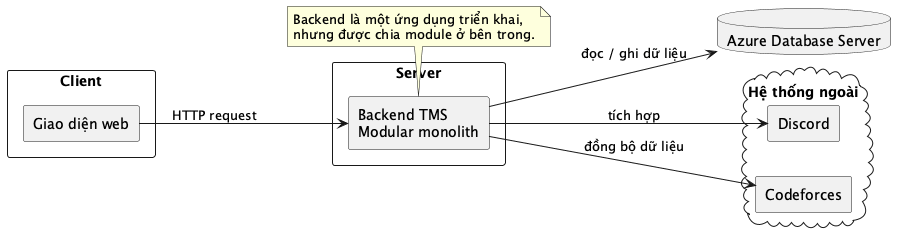
\includegraphics[width=0.86\textwidth,height=0.58\textheight,keepaspectratio]{diagrams/kieu-kien-truc.png}
    \caption{Kiểu kiến trúc được áp dụng trong hệ thống TMS}
\end{figure}

\subsection{Các thành phần chính}

\begin{figure}[H]
    \centering
    
\includegraphics[width=0.96\textwidth,height=0.68\textheight,keepaspectratio]{diagrams/cac-thanh-phan-chinh.png}
    \caption{Các thành phần chính và quan hệ phụ thuộc}
\end{figure}

Các thành phần chính được chia thành bốn nhóm để thể hiện rõ trách nhiệm và
ranh giới của từng phần trong hệ thống.

\textbf{Nhóm giao diện}
\begin{itemize}[leftmargin=*]
    \item \textbf{Giao diện web:} cung cấp màn hình thao tác cho giáo viên và quản trị viên.
    \item \textbf{API client:} đóng gói việc gửi HTTP request từ giao diện đến các endpoint backend.
\end{itemize}

\textbf{Nhóm backend}
\begin{itemize}[leftmargin=*]
    \item \textbf{Route:} nhận request, kiểm tra định dạng dữ liệu đầu vào và chuyển request vào controller tương ứng.
    \item \textbf{Controller:} điều phối request đã hợp lệ thành lời gọi use case, chuẩn hóa response trả về cho giao diện.
    \item \textbf{Security:} xác thực token, kiểm tra vai trò và kiểm tra phạm vi sở hữu dữ liệu.
    \item \textbf{Account module:} quản lý đăng nhập, hồ sơ, tài khoản giáo viên và định danh liên quan tài khoản.
    \item \textbf{Student module:} quản lý học sinh, ghi danh, chuyển lớp, rút khỏi lớp, lưu trữ và dữ liệu học sinh liên quan Discord.
    \item \textbf{Classroom module:} quản lý lớp học, lịch học, buổi học, điểm danh, Discord của lớp, thông báo và Gym.
    \item \textbf{Finance module:} quản lý giao dịch, khoản phí, số dư học sinh và báo cáo tài chính.
    \item \textbf{System module:} quản lý tài khoản giáo viên và cấu hình hệ thống dùng chung.
\end{itemize}

\textbf{Nhóm dữ liệu}
\begin{itemize}[leftmargin=*]
    \item \textbf{Azure Database Server:} lưu dữ liệu nghiệp vụ và dữ liệu đã đồng bộ từ hệ thống ngoài.
\end{itemize}

\textbf{Nhóm hệ thống ngoài}
\begin{itemize}[leftmargin=*]
    \item \textbf{Discord:} hỗ trợ định danh, guild, channel, tin nhắn và các chức năng lớp học liên quan Discord.
    \item \textbf{Codeforces:} hỗ trợ dữ liệu Gym, bài tập và bảng xếp hạng luyện tập.
\end{itemize}

Backend được chia theo ranh giới nghiệp vụ. Bảng dưới đây tóm tắt phạm vi của
các module chính.

\begin{longtable}{L{3.2cm} L{11.4cm}}
\toprule
\textbf{Module} & \textbf{Phạm vi trách nhiệm} \\
\midrule
\endhead
Account & Đăng nhập, hồ sơ người dùng, tài khoản giáo viên và các định danh liên quan tài khoản. \\
Student & Học sinh, ghi danh, chuyển lớp, rút khỏi lớp, lưu trữ học sinh và dữ liệu học sinh liên quan Discord. \\
Classroom & Lớp học, lịch học, buổi học, điểm danh, thiết lập Discord cho lớp, thông báo và Gym. \\
Finance & Giao dịch tài chính, khoản phí, số dư học sinh và báo cáo tài chính. \\
System & Chức năng quản trị hệ thống như quản lý tài khoản giáo viên và cấu hình bot Discord. \\
Security & Xác thực, phân quyền và kiểm tra phạm vi truy cập. Đây là lớp dùng chung, không phải module nghiệp vụ độc lập. \\
\bottomrule
\end{longtable}

Các module backend chạy trong cùng một ứng dụng. Khi cần dữ liệu hoặc hành vi
từ module khác, hệ thống ưu tiên điểm giao tiếp công khai thay vì phụ thuộc vào
chi tiết nội bộ của module đó.

\subsection{Thiết kế API endpoint}

Hệ thống sử dụng REST API.

\begin{figure}[H]
    \centering
    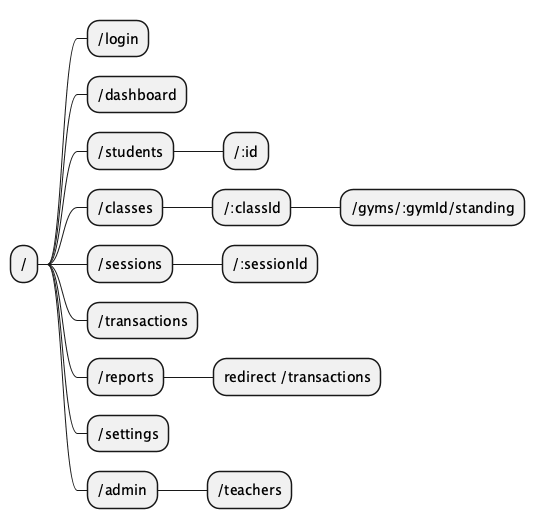
\includegraphics[width=0.96\textwidth,height=0.70\textheight,keepaspectratio]{diagrams/api-endpoint-frontend.png}
    \caption{Các endpoint giao diện hiện tại của frontend}
\end{figure}

\begin{figure}[H]
    \centering
    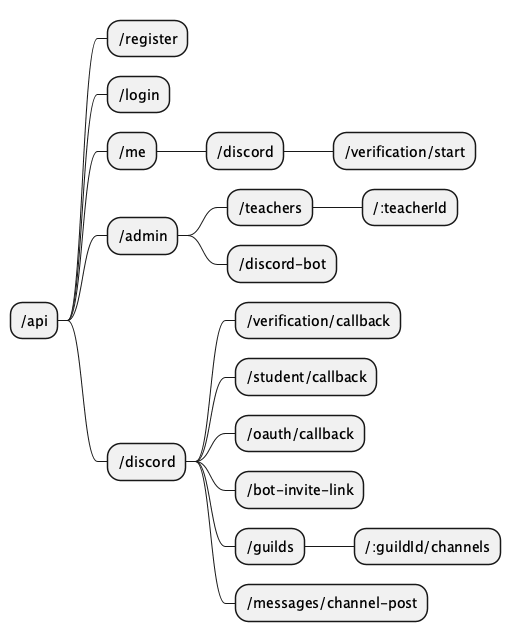
\includegraphics[width=0.96\textwidth,height=0.70\textheight,keepaspectratio]{diagrams/api-endpoint-backend-core.png}
      \caption{Các REST endpoint backend: tài khoản, quản trị và Discord}
\end{figure}

\begin{figure}[H]
    \centering
    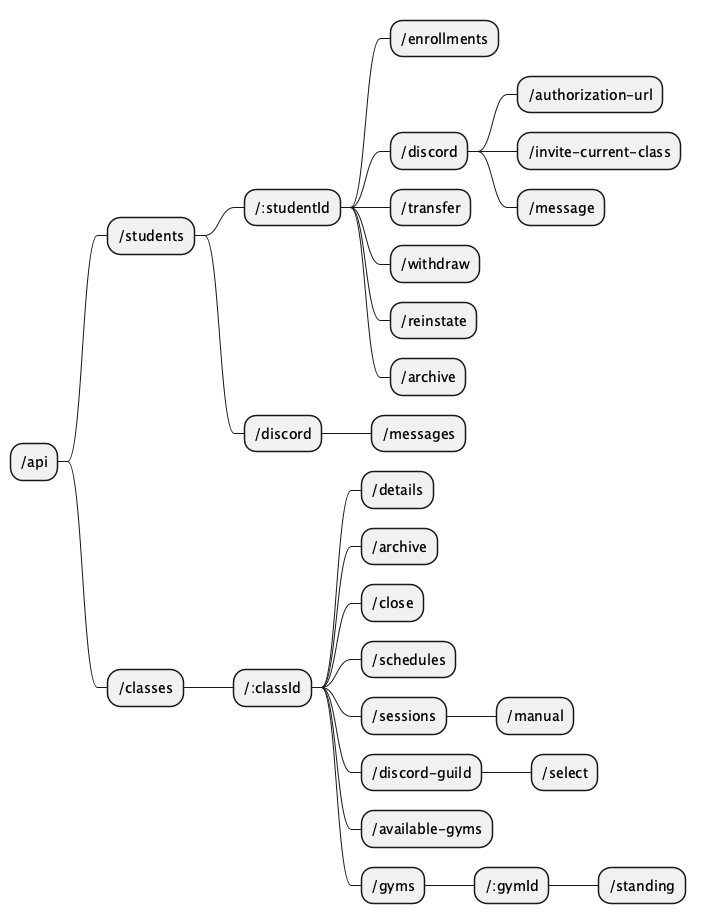
\includegraphics[width=0.96\textwidth,height=0.70\textheight,keepaspectratio]{diagrams/api-endpoint-backend-student-class.png}
    \caption{Các REST endpoint backend: học sinh và lớp học}
\end{figure}

\begin{figure}[H]
    \centering
    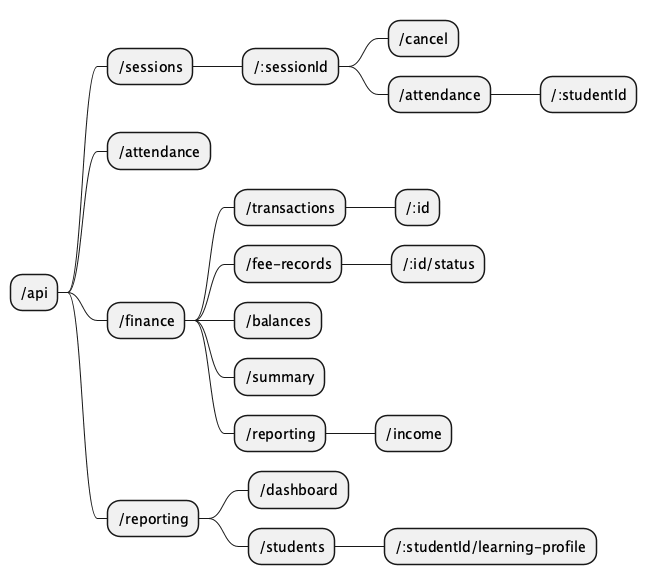
\includegraphics[width=0.96\textwidth,height=0.70\textheight,keepaspectratio]{diagrams/api-endpoint-backend-finance-reporting.png}
    \caption{Các REST endpoint backend: buổi học, điểm danh, tài chính và báo cáo}
\end{figure}

\subsection{Bảo mật và kiểm soát truy cập}

\begin{figure}[H]
    \centering
    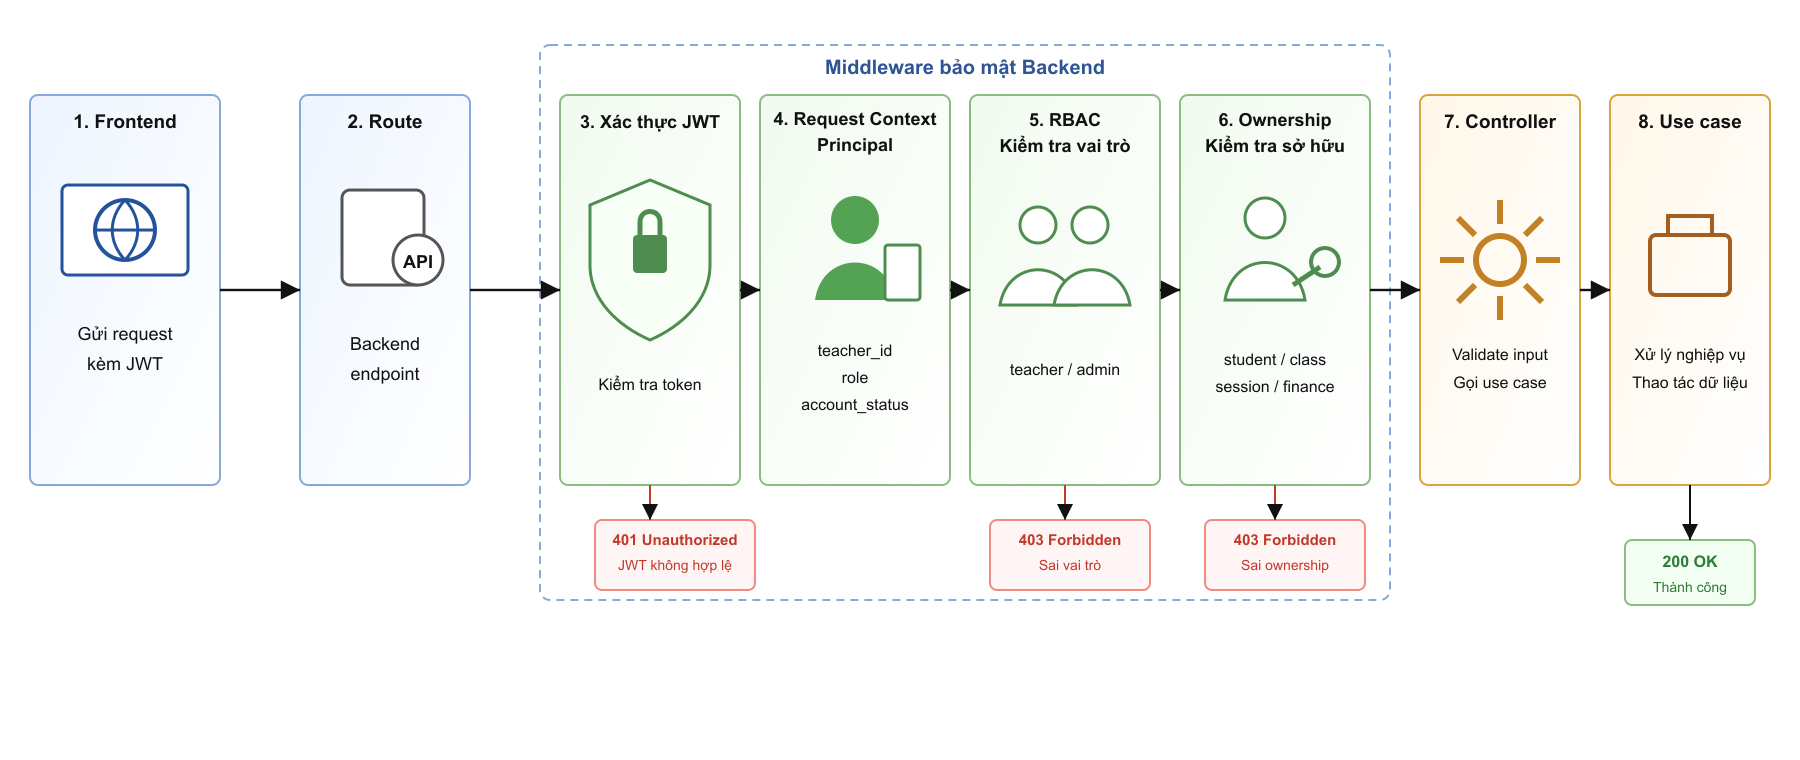
\includegraphics[width=0.96\textwidth,height=0.55\textheight,keepaspectratio]{diagrams/bao-mat-truy-cap.png}
    \caption{Luồng kiểm soát truy cập trước khi xử lý nghiệp vụ}
\end{figure}

Bảo mật được đặt ở lớp middleware của backend. Request từ frontend đi vào route
backend, sau đó phải lần lượt qua các bước xác thực JWT, tạo request context,
kiểm tra vai trò bằng RBAC và kiểm tra quyền sở hữu dữ liệu trước khi đến
controller.

\textbf{Quy tắc kiểm soát truy cập}
\begin{itemize}[leftmargin=*]
    \item Mọi request cần đăng nhập phải gửi JWT trong header \code{Authorization: Bearer <token>}.
    \item JWT authentication kiểm tra chữ ký, thời hạn và định dạng token. Nếu token thiếu hoặc không hợp lệ, request bị chặn với \code{401 Unauthorized}.
    \item Sau khi JWT hợp lệ, backend tạo principal trong request context, gồm \code{teacher\_id}, \code{role} và trạng thái tài khoản.
    \item RBAC kiểm tra vai trò có được phép đi vào route hay không. Admin được dùng route quản trị; teacher được dùng route nghiệp vụ của giáo viên. Sai vai trò bị chặn với \code{403 Forbidden}.
    \item Ownership check bảo đảm teacher chỉ truy cập dữ liệu thuộc phạm vi sở hữu của mình, gồm học sinh, lớp học, buổi học, hồ sơ tài chính và Gym được phân công. Sai phạm vi sở hữu cũng bị chặn với \code{403 Forbidden}.
\end{itemize}

\textbf{Mô tả luồng}
\begin{enumerate}[leftmargin=*]
    \item Frontend gửi HTTP request kèm JWT đến backend route.
    \item Route chuyển request qua middleware bảo mật.
    \item Middleware xác thực JWT và trích xuất principal.
    \item Hệ thống kiểm tra vai trò bằng RBAC.
    \item Với route truy cập dữ liệu theo giáo viên, hệ thống kiểm tra ownership.
    \item Request hợp lệ mới được chuyển đến controller và use case nghiệp vụ.
    \item Kết quả xử lý được trả về cho frontend.
\end{enumerate}

\subsection{Sơ đồ triển khai}

\begin{figure}[H]
    \centering
    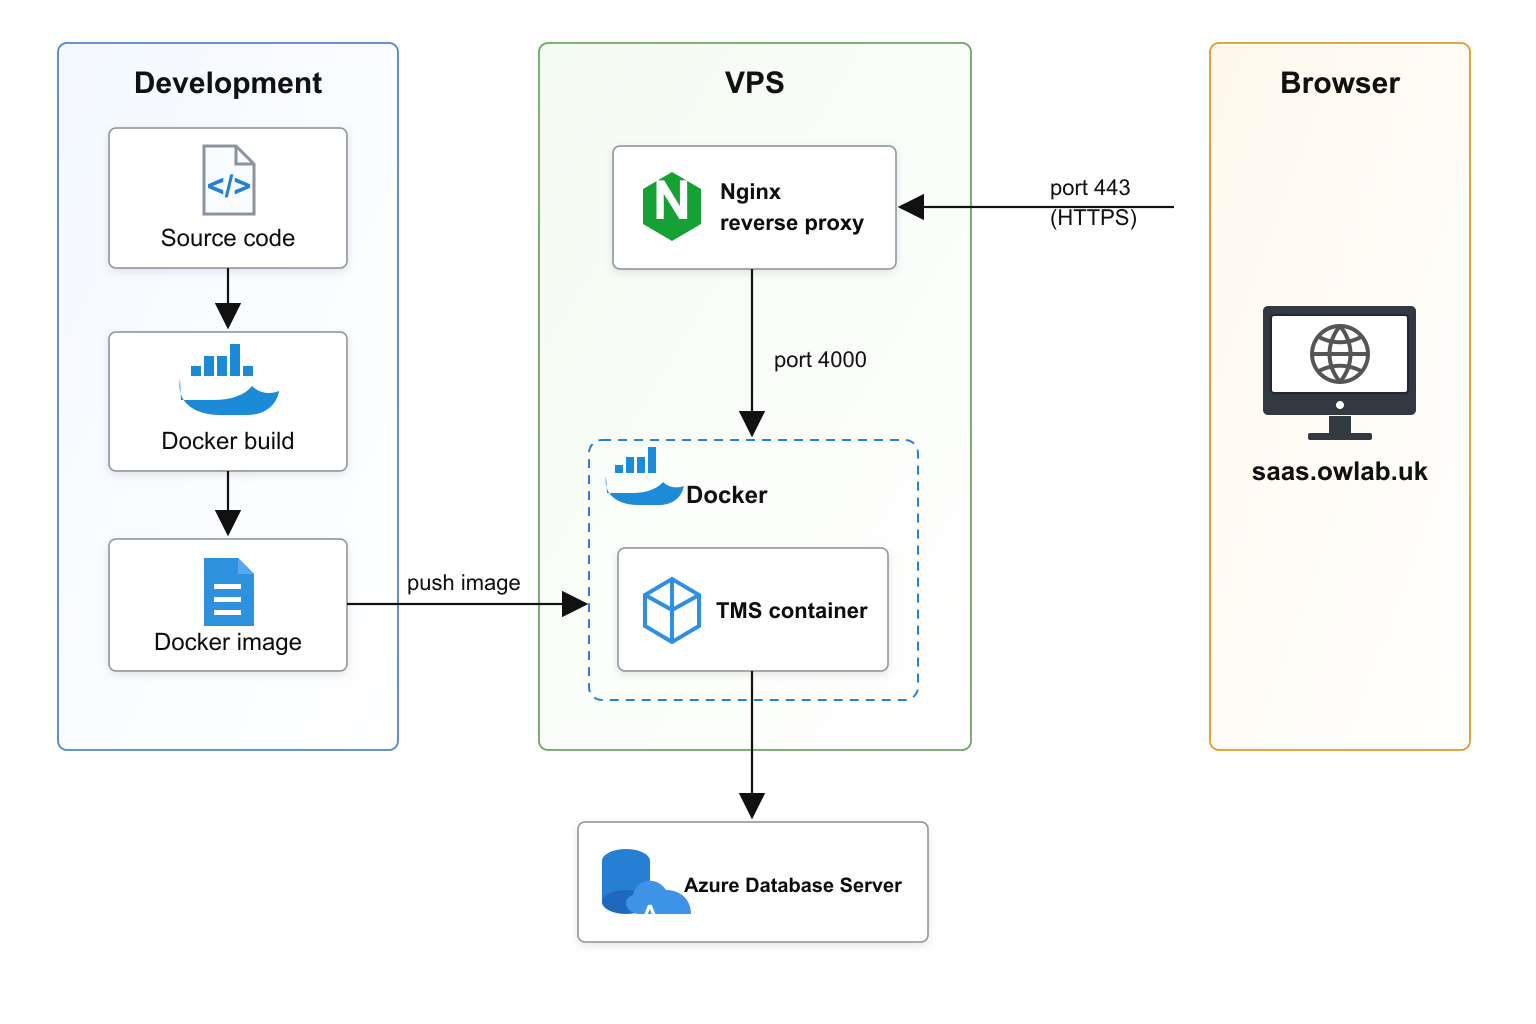
\includegraphics[width=0.92\textwidth,height=0.55\textheight,keepaspectratio]{diagrams/trien-khai-van-hanh.png}
    \caption{Sơ đồ triển khai phần mềm}
\end{figure}

\begin{enumerate}[leftmargin=*]
    \item Mã nguồn ở môi trường Development được build thành Docker image.
    \item Docker image được push từ môi trường Development sang VPS.
    \item Trên VPS, Docker chạy image này thành TMS container.
    \item Người dùng mở Browser và truy cập domain \code{saas.owlab.uk}.
    \item Request từ Browser đi vào VPS qua port 443.
    \item Nginx trên VPS nhận request ở port 443 và đóng vai trò reverse proxy.
    \item Nginx chuyển tiếp request vào TMS container qua port 4000.
    \item TMS container kết nối đến Azure Database Server để đọc và ghi dữ liệu TMS.
    \item TMS container xử lý request và trả kết quả ngược lại qua cùng đường đi.
\end{enumerate}

\end{document}
